\chapter{Software Implementierung}

\section{Systemarchitektur}

\section{Softwarearchitektur}


    %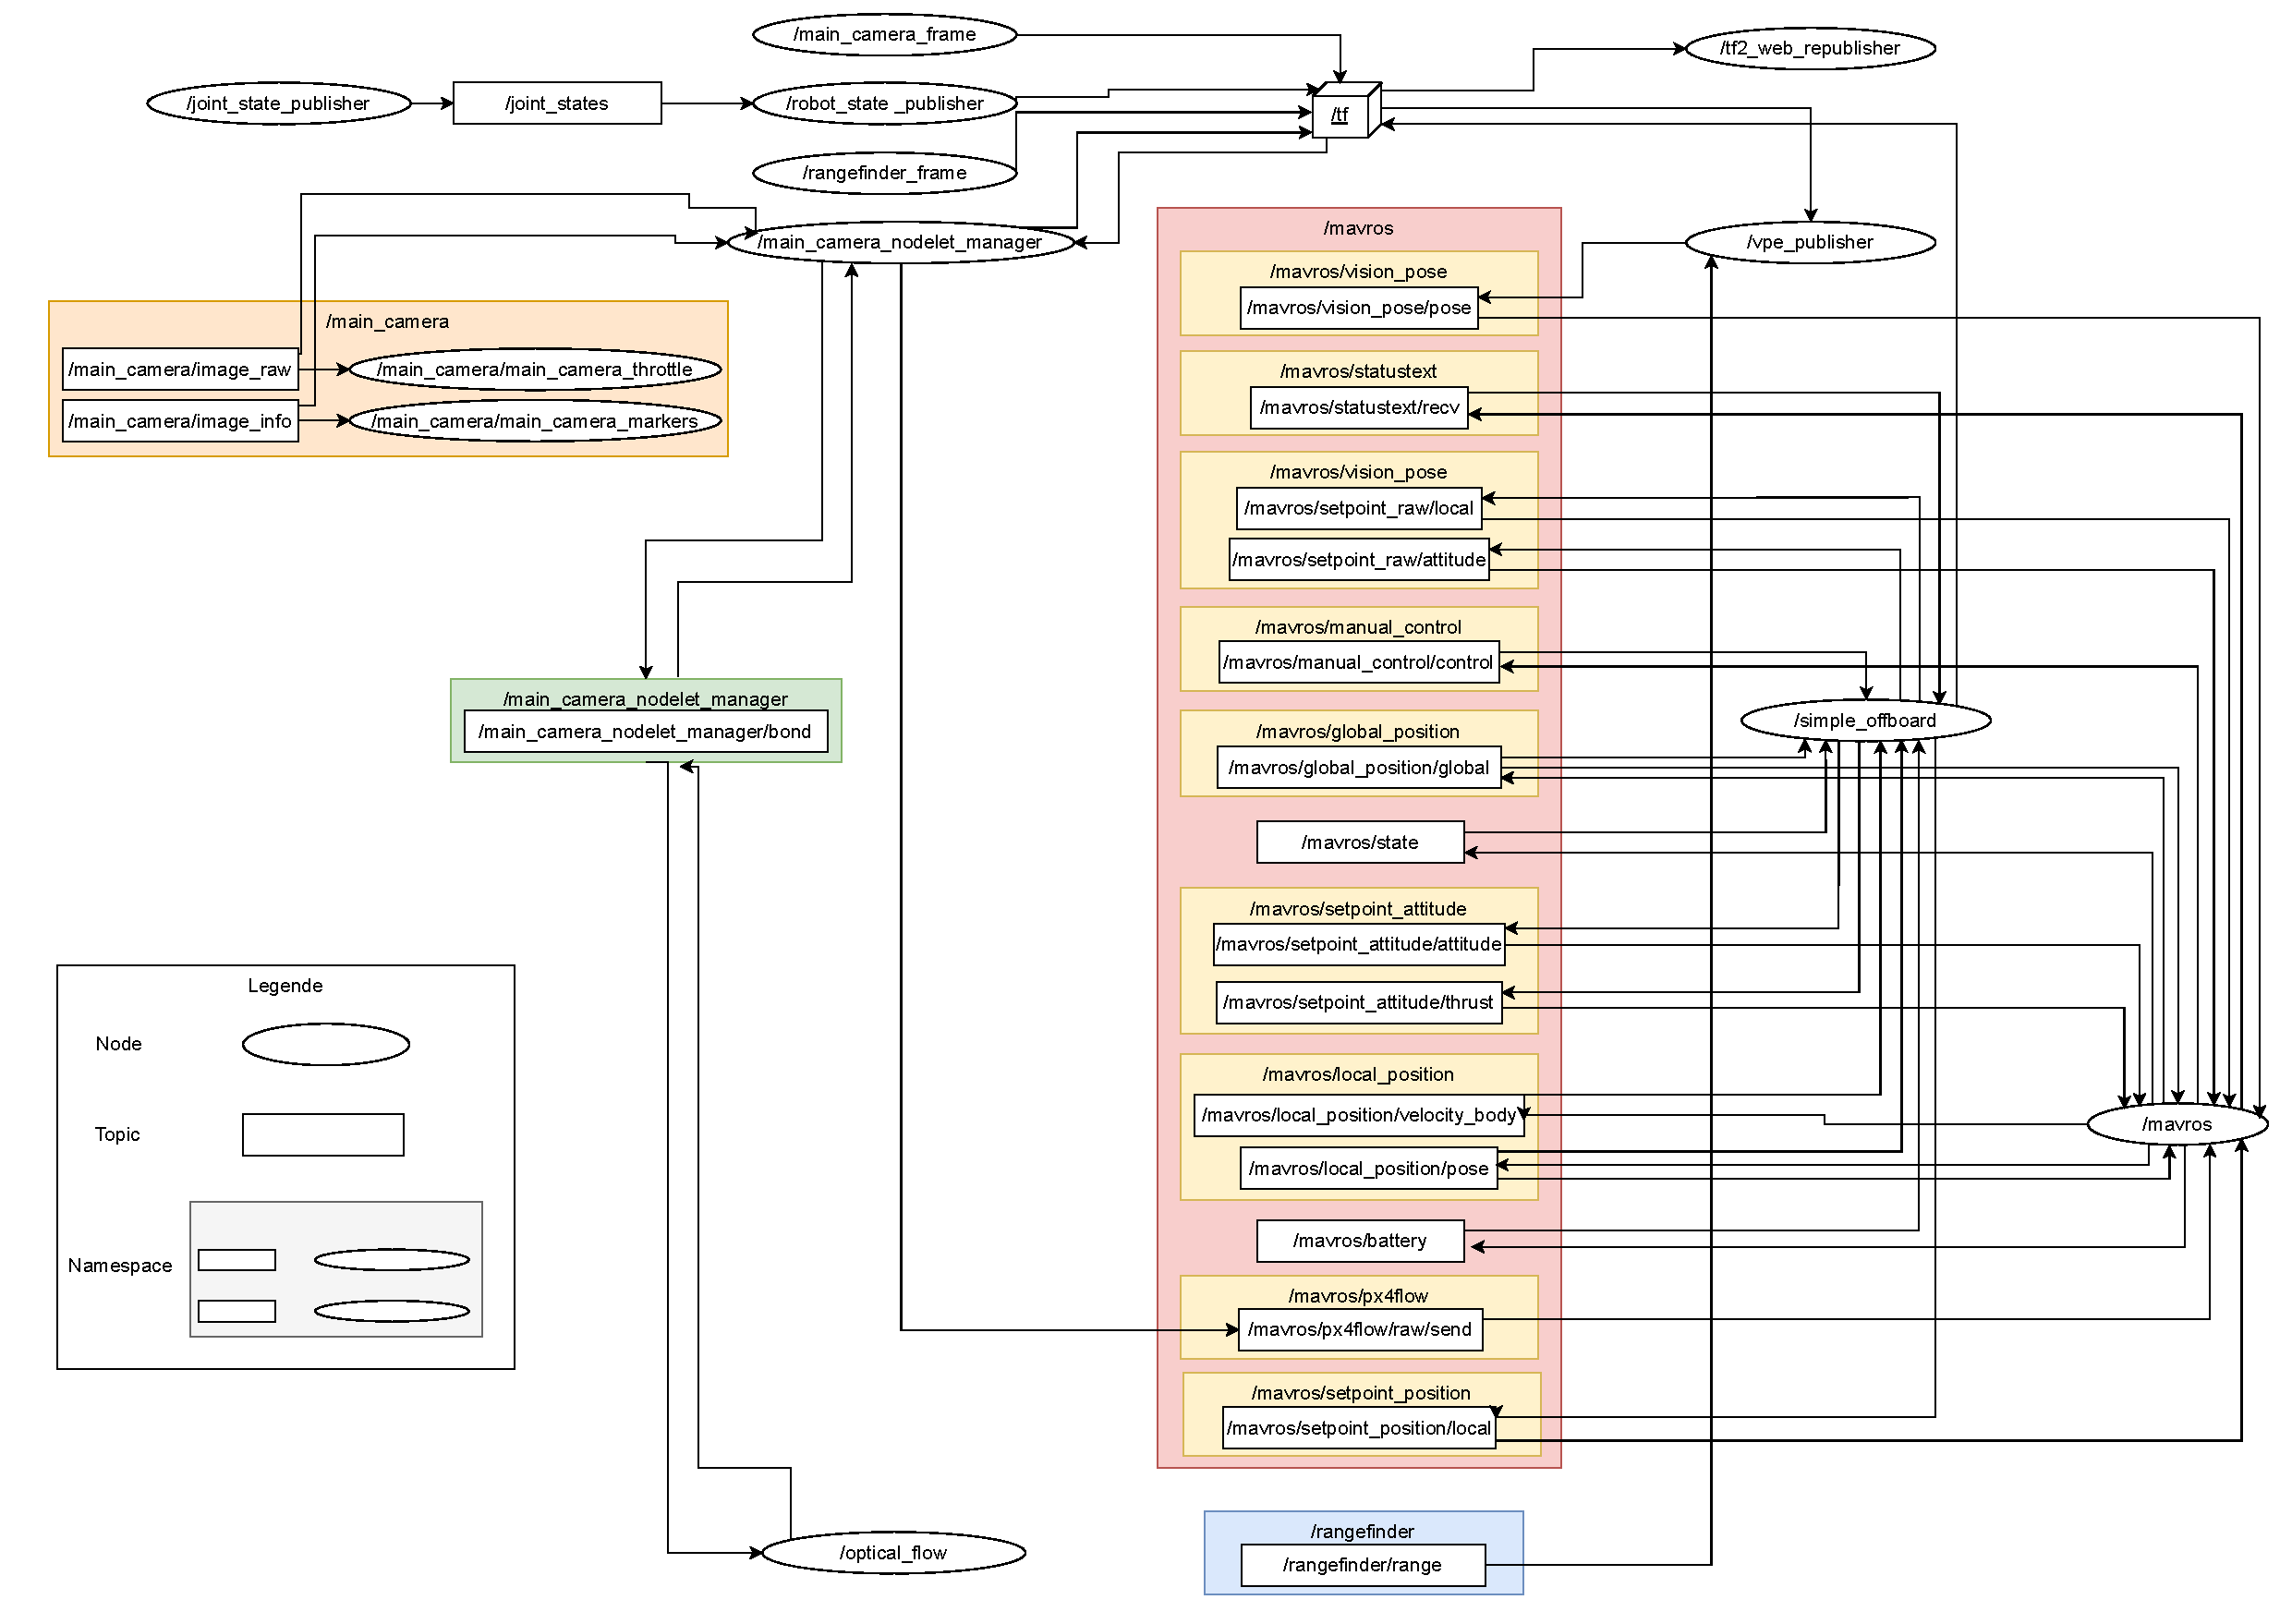
\includepdf[landscape=true]{images/graph_ros.pdf}
    %\caption[Übersicht ROS Nodes]{\label{img ros_nodes_graph} Übersicht ROS Nodes [eigene Darstellung]}
    \begin{landscape}
        \begin{figure}
            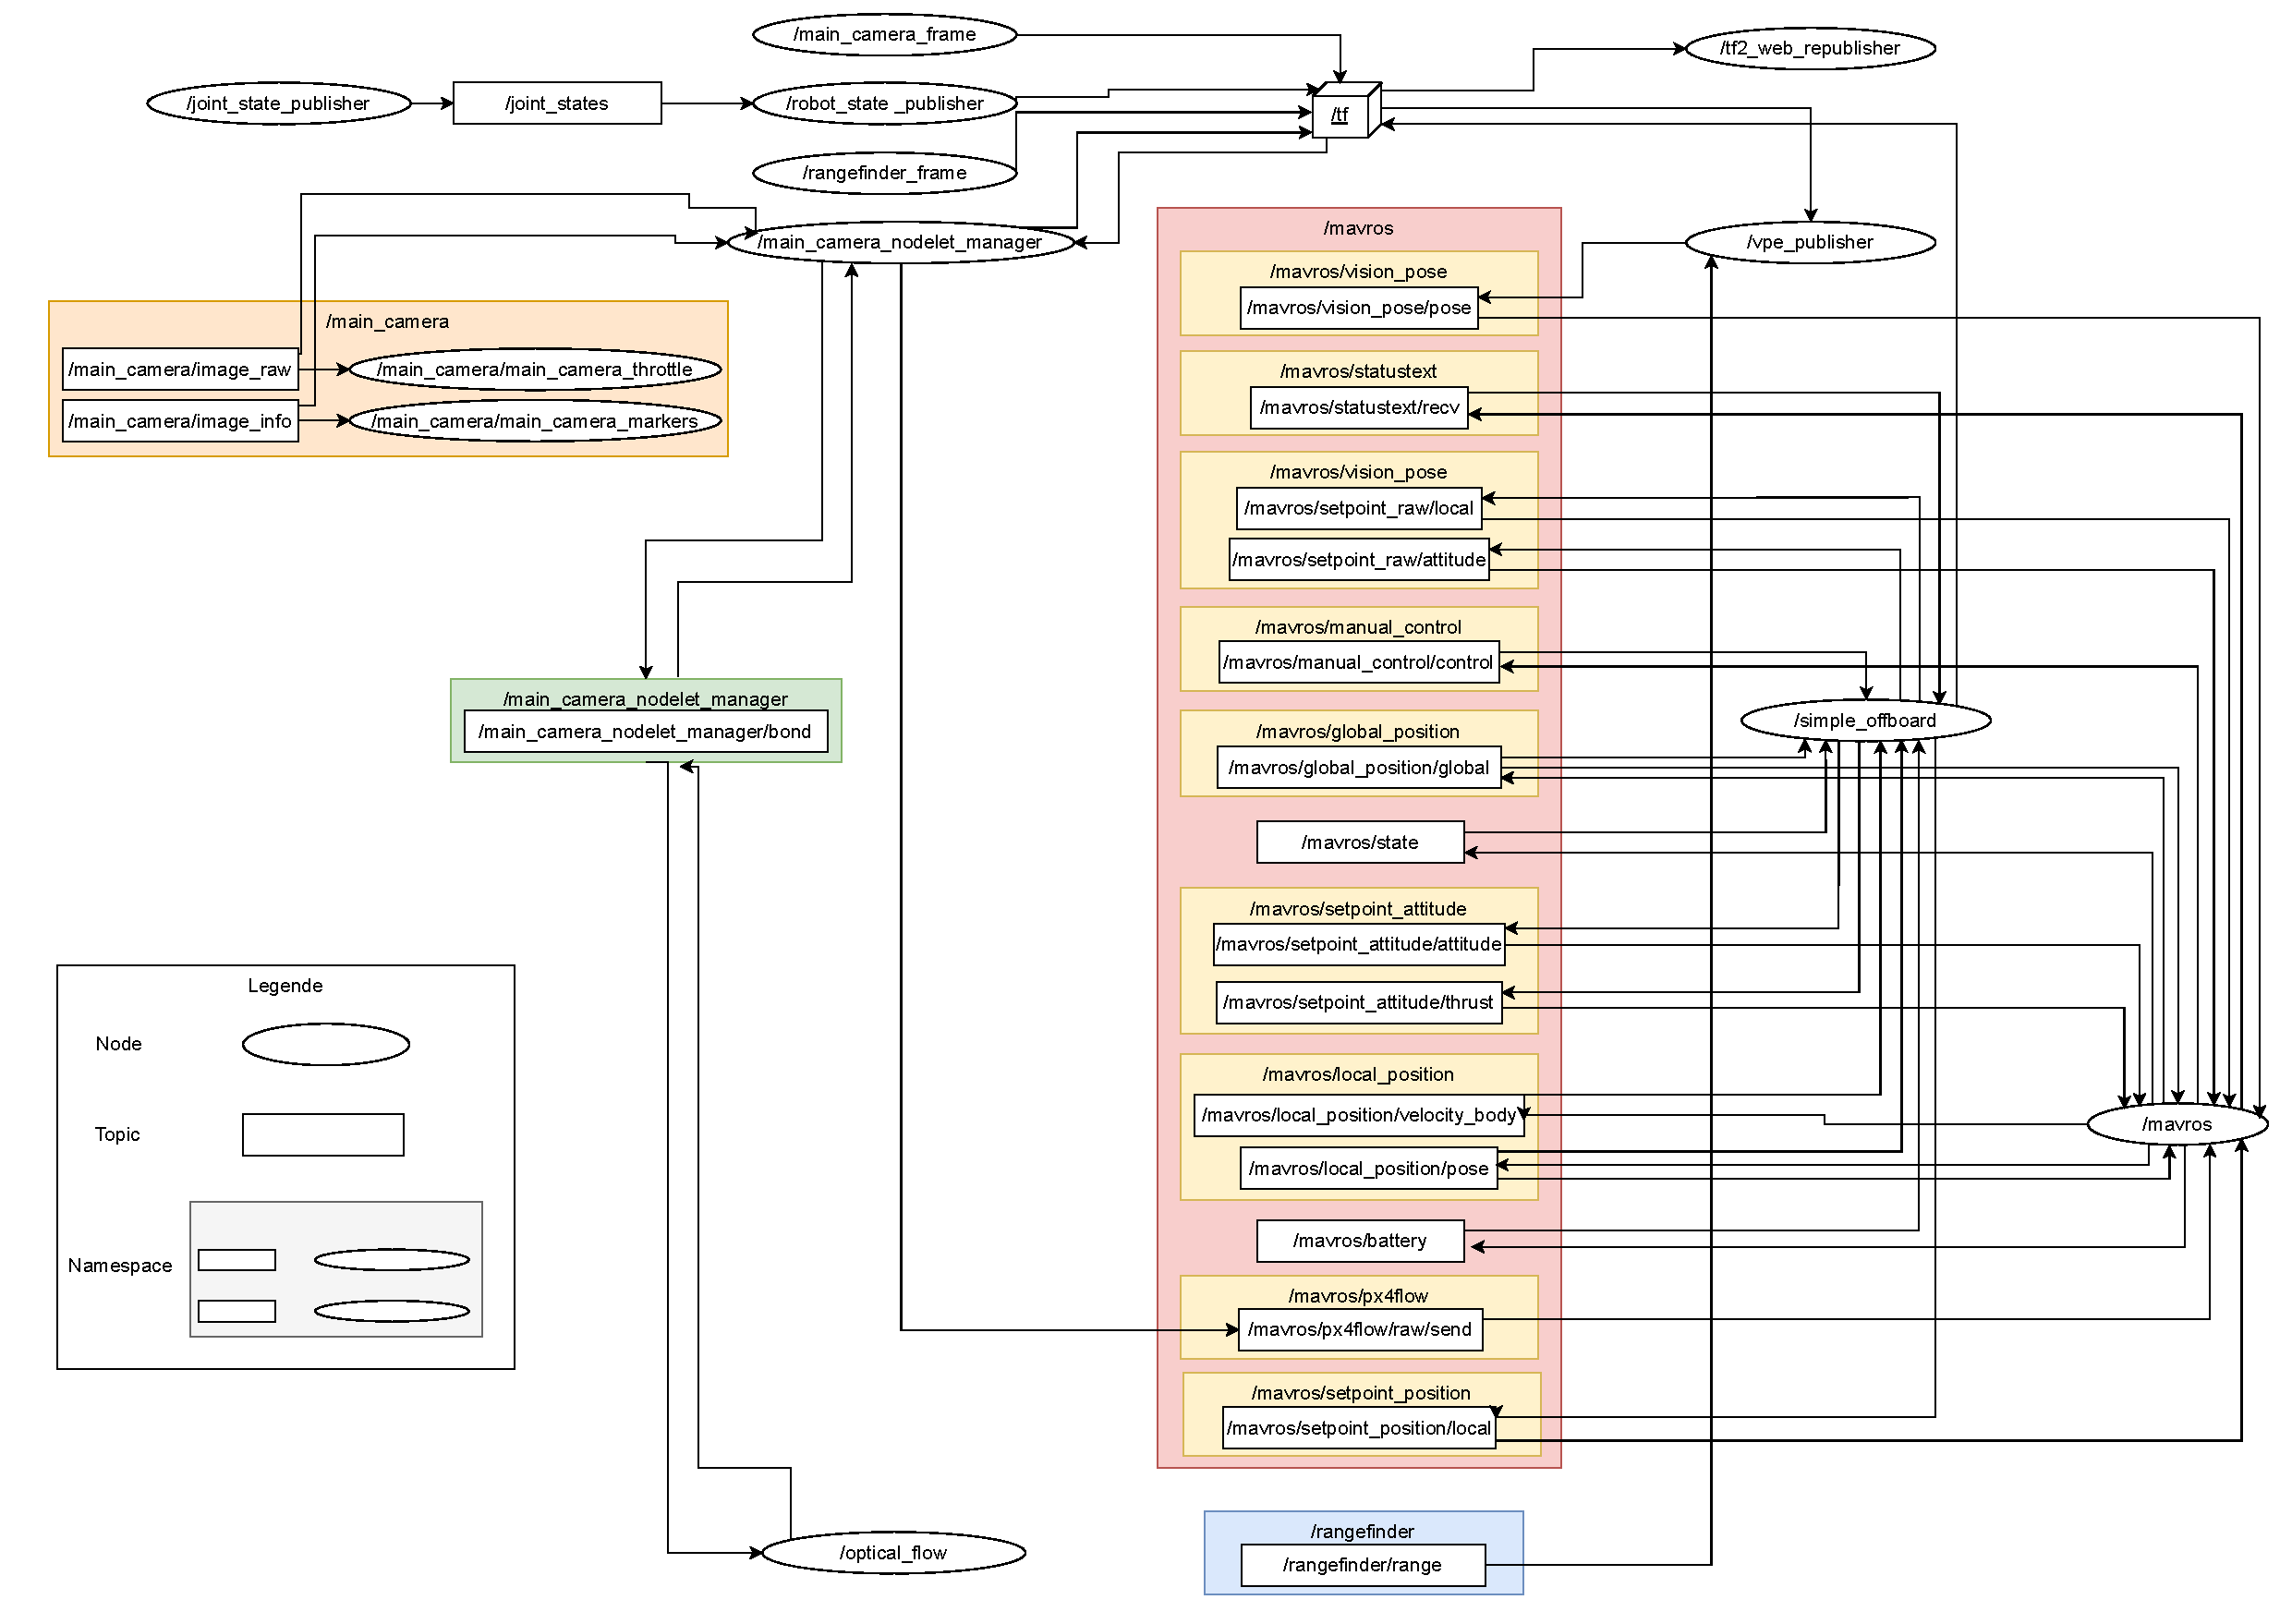
\includegraphics[width=\paperwidth,keepaspectratio]{images/graph_ros.pdf}
            \caption[Übersicht ROS Nodes]{\label{img ros_nodes} Übersicht ROS Nodes [eigene Darstellung]}
        \end{figure}
    \end{landscape}
\section{Kalibrierung der COEX Drohne}

\section{Drohnen Autopilot}

\subsubsection{PX4} \label{px4:subsection}
PX 4 ist eine Open-Source-Software, welche zur Steuerung verschiedener Arten von Fahrzeugen genutzt werden kann, hierzu zählen beispielsweise verschiedene Drohnenarten, sowie auch Fahrzeuge auf dem Boden und Unterwasserfahrzeuge.\\ Es kann zum einen für bereits flugfähigen Drohen eingesetzt werden. Aber es besteht auch die Möglichkeit eine neue Drohne in Verbindung mit PX4 zu bauen.\\
Für die Verwendung der PX4 Software kann QGroundControl (siehe Kapitel \ref{qGroundControl:subsection}) verwendet werden. \cite[vgl.][]{px4} \\
Der PX4-Flugstack wurde ursprünglich nur dür die Pixhawk-Hardware entwickelt, allerdings ist es heutzutage auch möglich diesen auf Linux-Computern und anderen Hardware einzusetzen. Wie es auch bei der Coex Clover Drohne mit dem Coex Pix umgesetzt wird. \\
Die Software setzt Sensoren, ein um den Zustand der Drohne zu bestimmen. Hierfür werden einige Sensoren vorausgesetzt, zu diesen zählen ein Gyroskop, ein Beschleunigungssensor, ein Magnetometer sowie ein Barometer. Zudem ist GPS empfohlen um weitere Modi nutzen zu können. \cite[vgl.][]{px4}

\subsubsection{QGroundControl}  \label{qGroundControl:subsection}
QGroundControl ist eine Software, welche vor allem für Drohnen mit einem PX4 aber auch anderen Flight Controller genutzt werden kann. Hierbei bietet es verschiedene Funktionen. Zum einen gehört hierzu die Konfiguration der einzelnen  Drohnen. Desweiteren ist es möglich mit der Software verschiedene Flugmodi auszuwählen, sowie diese dann auch während des Fluges zu überwachen, beispielweise durch die Anzeige der Flugposition auf einer Karte sowie auch deren Geschwindigkeit und andere Sensordaten.
Es ist auch möglich mit QGroundControl eine ganze Flugplanung zu machen, welche die Drohne daraufhin umsetzt. \cite[vgl.][]{qGroundControl}


\section{3D Modell}

    \subsection{3D Scan}

        \subsubsection{Microsoft HoloLens 2}

        \subsubsection{Azure Kinect \ac{DK}}

    \subsection{3D Modell Vorbereitung}

\section{Navigation}

\section{Simulation}



